\section{Ưu \& khuyết điểm của KMeans}
\subsection{Ưu điểm}
\begin{itemize}
	\item Thuật toán đơn giản, hiệu quả
	\item Sử dụng được với bộ số liệu lớn
\end{itemize}
\subsection{Khuyết điểm}
\begin{itemize}
	\item Cần phải xác định trước số lượng cluster. Trong thực tế, cần phải sử dụng thêm một số biện pháp giúp xác định giá trị K, chẳng hạn như elbow method.
	\item Thuật toán KMeans không đảm bảo tìm được nghiệm tối ưu toàn cục nên nghiệm cuối cùng phụ thuộc rất nhiều vào các centroid ban đầu.\\
	\begin{figure}[h]
		\centering
		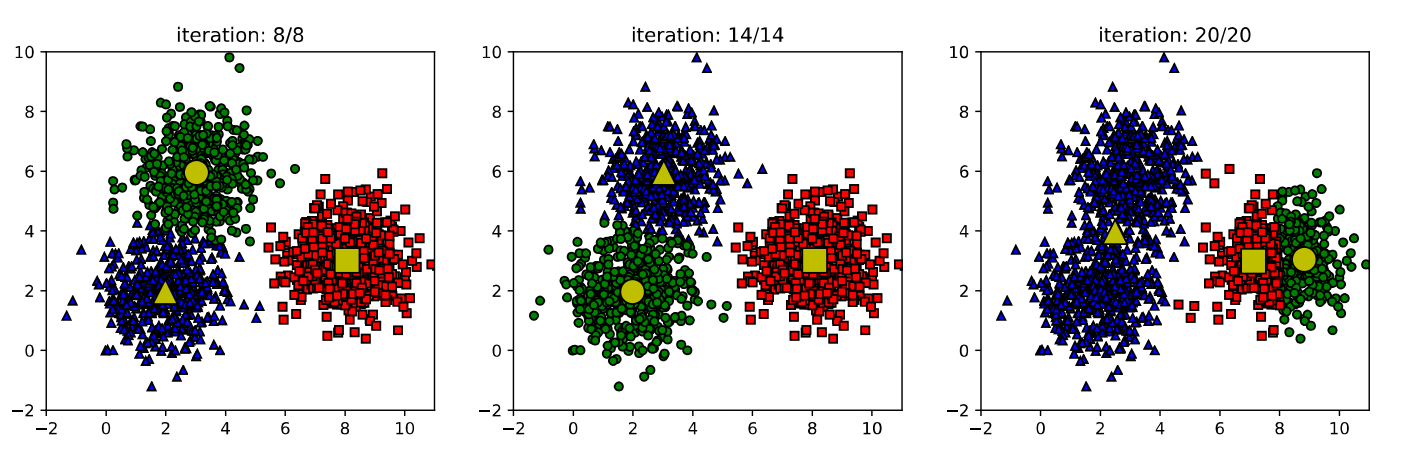
\includegraphics[width=0.7\linewidth]{img/disad_1}
		\caption{Các nghiệm khác nhau do khởi tạo ban đầu khác nhau}
	\end{figure}
	\item Các cluster cần phải có số lượng điểm gần bằng nhau\\
	\begin{figure}[h]
		\centering
		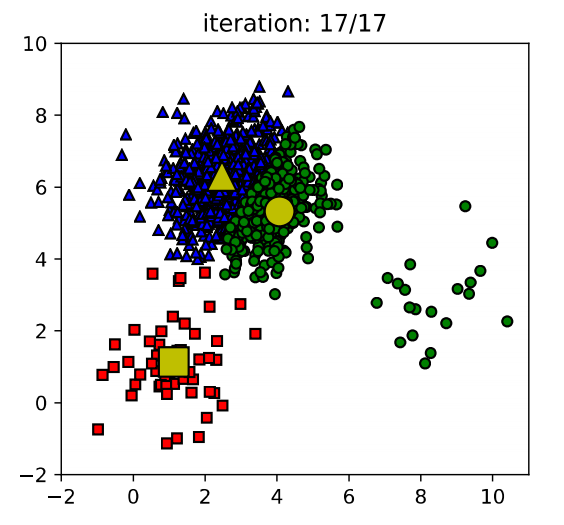
\includegraphics[width=0.3\linewidth]{img/disad_2}
		\caption{Các nghiệm trong cluster này bị nhầm vào cluster khác}
	\end{figure}
	\item Các cluster cần có dạng hình tròn (cầu)	
	\begin{figure}[h]
		\centering
		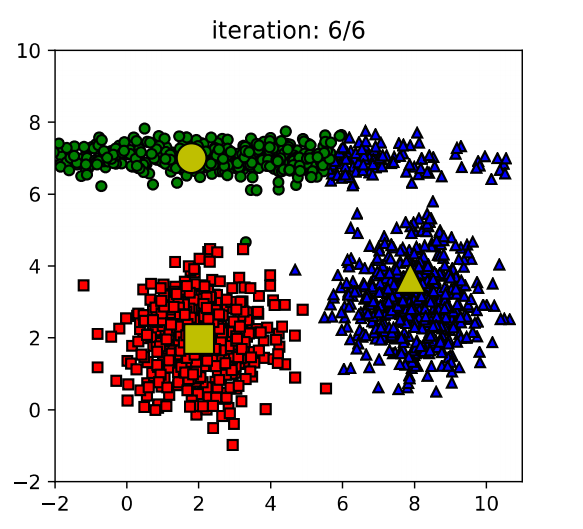
\includegraphics[width=0.3\linewidth]{img/disad_3}
		\caption{Các nghiệm trong cluster này bị nhầm vào cluster khác}
	\end{figure}
	\item Centroid có thể bị xê dịch bởi các ngoại lệ, hoặc các ngoại lệ có thể có cụm riêng thay vì bị bỏ qua.
	\item Cho kết quả sai khi một cluster này bị bao bọc bằng một cluster khác
	\begin{figure}[h]
		\centering
		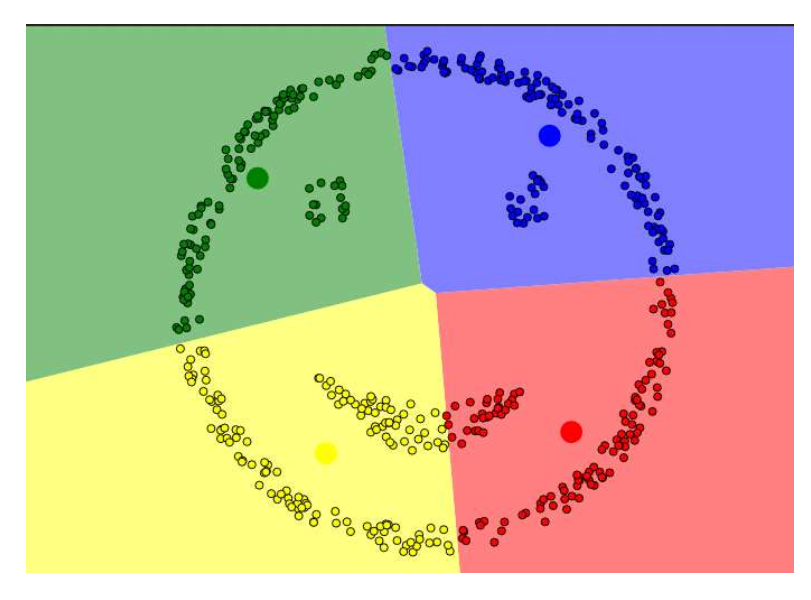
\includegraphics[width=0.7\linewidth]{img/disad_4}
		\caption{KMeans chia mặt làm 4 phần thay vì gom chung các bộ phận trong khuôn mặt thành 1 cụm}
	\end{figure}	
\end{itemize}
\newpage